\documentclass[a4paper,french]{paper}
\usepackage{../../_latex_assets/villemejane_iogs_ceti}

%Informations about this document 
%------------------------------------------
\def\module{Conception Electronique pour le Traitement de l'Information}
\def\moduleAbrege{5N-027-SCI / CéTI}
\def\annee{}

\def\titre{Bloc 4 / Systèmes et asservissement}
\author{Julien VILLEMEJANE}

\subtitle{Bloc4}
\institution{LEnsE / Institut d'Optique Graduate School}

\title{\titre}
\begin{document} 
%Beginning First Page. 
%------------------------------------------
\enteteThematiqueObligatoire{}

%Beginning Content. 
%------------------------------------------

\textbf{Objectifs}

Ce bloc de TD va vous permettre de découvrir un autre outil de calcul numérique, \textbf{MatLab} et son extension graphique \textbf{SimuLink} dans le cadre de l'\textbf{analyse de systèmes} pouvant se mettre sous forme d'une fonction de transfert.

\textbf{Ressources}

Pour l'ensemble des missions suivantes, vous pouvez vous inspirer des tutoriels situés à l'adresse suivante :

http://lense.institutoptique.fr/matlab/ 

\bigskip

%%%%%%%%%%%%%%%%%%%
\encadreTDExo{1 - Modéliser et simuler un système du premier ordre}{
De manière graphique, à l'aide de \textbf{Simulink}, saisissez le schéma suivant :


Réalisez ensuite la simulation de ce système en boucle ouverte,  
}


Idée 2 : Simulink - Système H(s) 2e ordre + Marges + Rebouclage (transimpédance)

Idée 3 : Simulink - Système H(s) 3e ordre + Bode + Rebouclage + Instabilité

Idée 4 : Matlab - tf + step + impulse + bode + FFT(impulse) sur système 2e ordre 

Idée 5 : Matlab - Système H(s) 3e ordre + Marges + Instabilité


%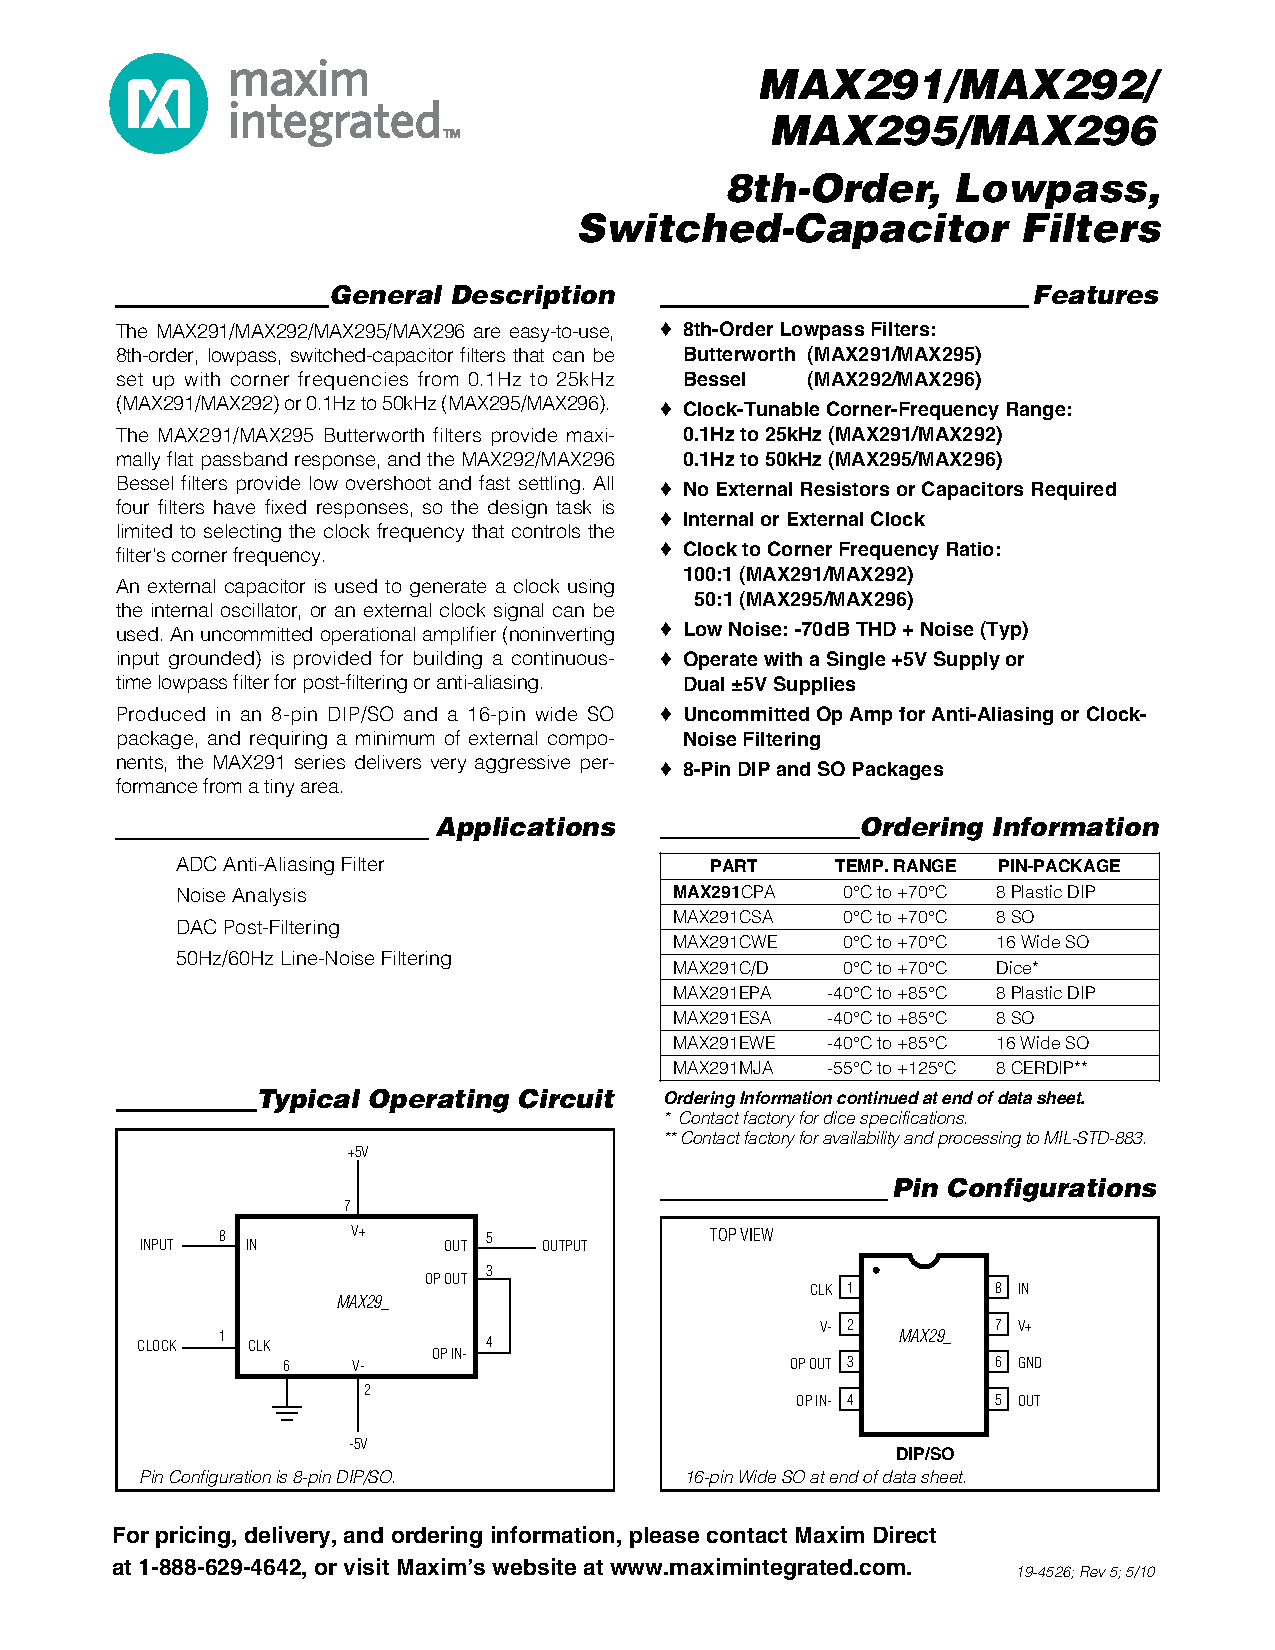
\includepdf[pages=-]{doc/MAX296.pdf}

\end {document}